\chapter{Transient flow and heat equations -- the Rayleigh-Benard instability}

\modinfo{Directory}{RayleighBenardGUI}
\modinfo{Solvers}{\Idx{HeatSolve}, \Idx{FlowSolve}}
\modinfo{Tools}{\Idx{ElmerGUI}}
\modinfo{Dimensions}{2D, Transient}

\subsection*{Case definition}

%\begin{flushleft}
This tutorial is about simulating the developing of the
Rayleigh-Benard instability in a rectangular domain  (Figure
\ref{fg:rb_geometry}) of dimensions 0.01 m height and 0.06 m
length. The simulation is performed with water and the material
parameters of water required by the Elmer model are presented in Table \ref{tb:matpar}. The
temperature difference between the upper and lower boundary is set to
0.5 so that lower one has the temperature of  283.5 K and the upper
one has the temperature of 283 K.


The density of water is inversely proportional to its
temperature. Thus, heated water starts to flow upwards, and colder
downwards due to gravity.  In this case we assume that the
\Idx{Boussinesq} approximation is valid for thermal incompressible
fluid flow. In other words, the density of the term $\rho$$\vec{f}$ in
the incompressible Navier-Stokes equation can be redefined by the
Boussinesq approximation
\begin{displaymath}
\rho = {\rho}_0(1-\beta(T-{T}_0))
\end{displaymath}
where $\beta$ is the heat expansion coefficient and the subscript 0 refers to a reference sate.


\begin{figure}[h]
\centering
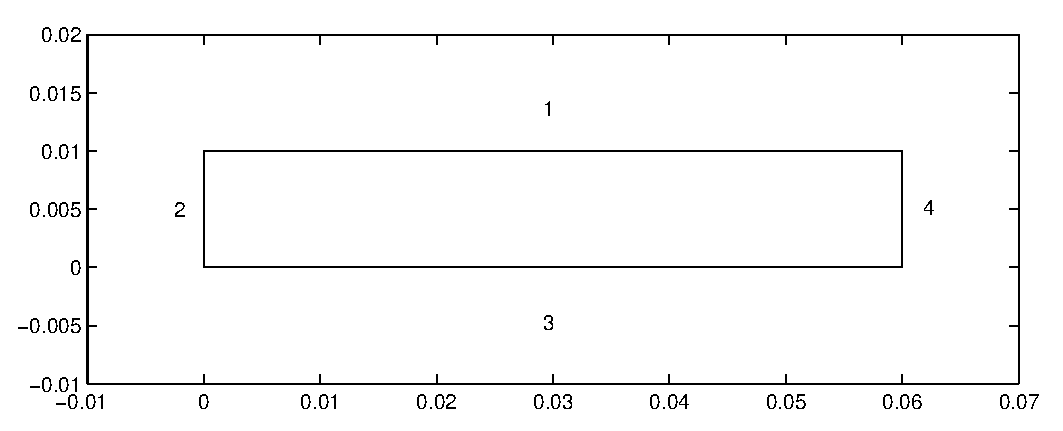
\includegraphics[width=150 mm, height=55 mm]{rb_geometry}
\caption{Domain.}\label{fg:rb_geometry}
\end{figure}  


\begin{table}[h]
\caption{Material parameters.}
\label{tb:matpar}
\begin{center}
\begin{tabular}{ll} \hline
parameter  & value \\ \hline
density & 1000 kg/m$^{3}$ \\
viscosity & 1040e-6 Ns/m$^{2}$ \\
heat capacity & 4190 J/(kg$\cdot$K) \\
heat conductivity & 0.6 W/(m$\cdot$K)       \\
heat expansion coefficient & 1.8e-4 K$^{-1}$      \\ 
reference temperature & 283 K       \\ \hline
\end{tabular}
\end{center}
\end{table}


\subsection*{Solution procedure}

The mesh is given in ElmerGrid format in file \texttt{box.grd}, load this file.
\ttbegin
File 
  Open -> box.grd
\ttend
You should obtain your mesh and may check that it consists of 3036 bilinear elements.

There is a possibility to divide and unify edges to simplify the case definition in the future.
\ttbegin
Choose (left wall + right wall (Ctrl down)) -> unify edge
\ttend

After we have the mesh we start to go through the Model menu from the top to bottom. 
In the Setup we choose things related to the whole simulation such as file names, 
time stepping, constants etc.
The simulation is carried out in 2-dimensional cartesian
coordinates. 2nd order bdf time-stepping method is selected with 200 steps
and with step size of two seconds.
\ttbegin
Model
  Setup 
    Simulation Type = Transient
    Steady state max. iter = 20
    Time Stepping Method = bdf
    BDF Order = 2
    Time Step Intervals = 200
    Time Step Sizes = 2.0
    Gravity = ...
\ttend
In the equation section we choose the relevant equations and paremeters related to their solution. 
In this case we'll have one set of equations (named ``Natural Convection'') which consists of the heat equation
and of the Navier-Stokes equation.

When defining Equations and Materials it is possible to assign the to bodies immediately, or to use mouse
selection to assign them later. In this case we have just one body and therefore its easier to assign 
the Equation and Material to it directly.
It is important to select the 
convection to be computed since that couples the velocity field to the heat equation.

The system may include nonlinear iterations of each equation and steady state iterations 
to obtain convergence of the coupled system. It is often a good idea to keep the number of 
nonlinear iterations in a coupled case low. Here we select just one nonlinear iteration
for both equations.
For the linear system solvers we are happy to use the defaults. One may however, try out different
preconditioners (ILU1,\ldots) or direct Umfpack solver, for example.
\ttbegin
Model
  Equation
    Name = Natural Convection
    Apply to Bodies = 1
    Heat Equation
      Active = on
      Convection = Computed
      Edit Solver Setting
        Nonlinear System
          Max. iteations = 1
    Navier-Stokes 
      Active = on
      Edit Solver Setting
        Nonlinear System
          Max. iteations = 1
\ttend        
The Material section includes all the material parameters.
They are divided to generic parameters which are direct properties of the material
without making any assumptions on the physical model, such as the mass. Other properties assume
a physical law, such as conductivities and viscosity.      
\ttbegin
Model
  Material
    Name = Fluid
    Apply to Bodies = 1 
    General    
      Density = 1000
      Heat Capacity = 4190
      Reference Temperature = 283
      Heat expansion Coeff. = 1.8e-4
    Heat Equation
      Heat Conductity = 0.6
    Navier-Stokes
      Viscosity = 1.04e-3
\ttend

A Body Force represents the right-hand-side of a equation. It is generally 
not a required field for a body. In this case, however, we apply the bouyancy resulting from
heat expansion as a body force to the Navier-Stokes equation.
\ttbegin
Model
  Body Force
    Name = Boyancy
    Apply to Bodies = 1
    Navier Stokes
      Boussinesq = on
\ttend    

Initial conditions should be given to transient cases. In this case we choose a constant Temperature field
and a small initial velocity. 
\ttbegin
Model
  Initial Condition 
    Name = Initial Guess
    Heat Equation
      Temperature = 283
    Navier-Stokes
      Velocity 1 = 1.0e-9
      Velocity 2 = 0.0
\ttend

Only one boundary condition may be applied to each boundary and therefore all the 
different physical BCs for a boundary should be grouped together. In this case the
Temperature and Velocity. The side walls are assumed to be adiabatic.
\ttbegin
Model
  BoundaryCondition
    Name = Bottom
    Heat Equation
      Tempateture = 283.5
    Navier-Stokes 
      Velocity 1 = 0.0
      Velocity 2 = 0.0
 
    Name = Top
    Heat Equation
      Tempateture = 283
    Navier-Stokes 
      Velocity 1 = 0.0
      Velocity 2 = 0.0
 
    Name = Sides
    Navier-Stokes 
      Velocity 1 = 0.0
      Velocity 2 = 0.0
\ttend   

The boundary conditions may also be set in the Boundary condition menu, or 
by clicking with the mouse. Here we use the latter approach as that spares us of the 
need to know the indexes of each boundary.
\ttbegin
Model
  Set boundary properties
    Choose Bottom -> set boundary condition Bottom
    Choose Top -> set boundary condition Top
    Choose Sides -> set boundary condition Sides
\ttend

After the case have been set-up we may check that all edges and surfaces have been assigned 
boundary condition, or an equation and material parameters.
\ttbegin
View
  Select defined edges 
  Select defined surfaces
\ttend 
If everything is set we may continue, otherwise one should go back to check what data is missing.
\ttbegin
View
  Reset model view
\ttend

For the execution 
ElmerSolver needs the mesh files and the command file. We have know basically defined
all the information for ElmerGUI to write the command file. After writing it we may also visually 
inspect the command file.
\ttbegin
Sif 
  Generate
  Edit -> look how your command file came out  
\ttend

Before we can execute the solver we should save the files in a directory. Both the command file and
the mesh file will be saved simultaneously to the destination directory.
\ttbegin
File 
  Save As
\ttend

After we have succefully saved the files we may start the solver
\ttbegin
Run
  Run solver
\ttend
A convergence view automatically pops up showing relative changes of each iteration.
When there are some results to view we may start the postprocessor also
\ttbegin
Run
  Run postprocessor
\ttend


\subsection*{Results}

Due to the number of the time-steps the simulation may take around ten minutes.
You may inspect the results with ElmerPost as the time-steps are computed, or
wait until all timesteps have been computed. 
When opening the result file using ElmerGUI ElmerPost only opens the first time-step.
Therefore it is important to reopen the file and load the time-steps of interest.
Pressing the button $\bf{All}$ selects all the calculated time steps.
A video of the results can be viewed by selecting the option $\bf{Timestep}$ 
$\bf{Control}$ and pressing the button $\bf{Loop}$ under the $\bf{Edit}$ menu.

In Figures \ref{fg:rb_temp} and \ref{fg:rb_vel} the obtained temperature 
distribution and the velocity vectors are presented. 
The maximum velocity in the system should be about 0.4 mm/s. 

\begin{figure}[h]
\centering
\includegraphics[width=150 mm, height=50 mm]{rb_temp}
\caption{Temperature distribution at 260 s.}\label{fg:rb_temp}
\end{figure} 

\begin{figure}[h]
\centering
\includegraphics[width=150 mm, height=70 mm]{rb_vel}
\caption{Velocity vectors at 260 s.}\label{fg:rb_vel}
\end{figure} 





